By this point in the analysis all the selections have been finalised and discussed.
Furthermore, clear definitions for tag-$B$ mesons that properly kinematically constrain \BtoXsgamma are presented, such that \EB is evaluated accurately.
However, as can be seen \Cref{fig:spectrum_after_optimisation}, even though continuum and $\BB$ backgrounds is suppressed heavily compared to the \EB distributions that was begun with (\Cref{fig:spectrum_after_reco}),
there is still a significantly larger number of background processes than \BtoXsgamma signal events.
Many of these, particularly continuum background, originate from incorrect tag-$B$ mesons (see \Cref{fig:good_tag_definitions}) and can therefore be estimated in data using an \Mbc fitting procedure.
In this section, a thorough overview of the \Mbc fit will be presented which will extract the counts of good-$B$ tags in different \EB intervals.

\subsection{Components in the dataset}\label{sec:fitting_components}

There are three types of events in \epem collision dataset following all the selections described so far:
\begin{itemize}
    \item Generic-\BB (including \BtoXsgamma) that are tagged with a good tag-$B$;
    \item Generic-\BB (including \BtoXsgamma) that are tagged with a misreconstructed tag-$B$;
    \item Photons candidates originating in \epem\ra\qqbar.
\end{itemize}
These three components are referred to as `peaking', `combinatorial \BB' and `continuum' throughout this \Cref{sec:fitting_mbc}.
The fitting model is prepared to describe these components and extract the number of tag-$B$ candidates that corresponds to the `peaking' component.

Conventionally, \Mbc distributions are often fitted using a Crystal Ball, and ARGUS distribution. 
The former is a Gaussian central part, that has a low end tail replaced with a polynomial. 
The latter, is a probability distribution specifically defined to describe continuum background particle distributions in B factory experiments.

\todo[inline]{need equations here, crystal ball, argus, chebyshev and define pull and also in the caption below.}

\begin{figure}[htbp!]
    \subcaptionbox{\label{fig:good_tags_fit}}{
        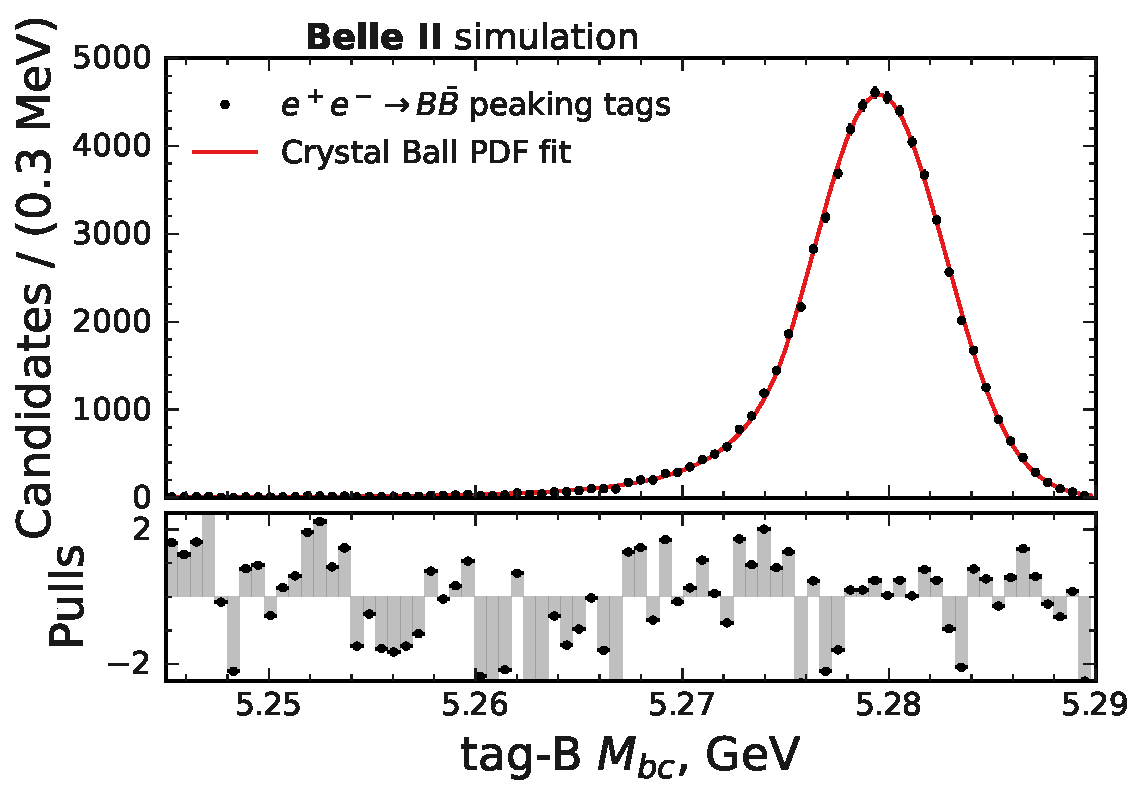
\includegraphics[width=0.3\textwidth]{figures/fitting/mbc_good_tags_fit.pdf}
    }
    \subcaptionbox{\label{fig:combinatorial_tags_fit}}{
        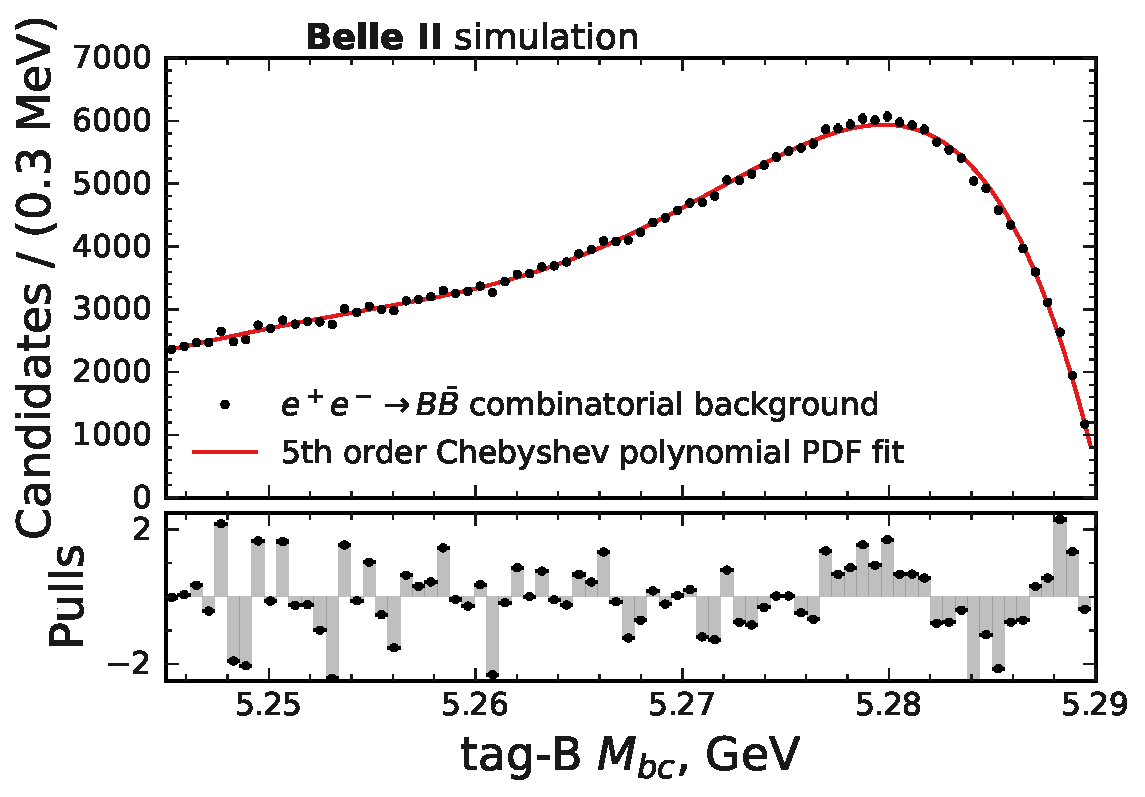
\includegraphics[width=0.3\textwidth]{figures/fitting/mbc_combinatorial_tags_fit.pdf}

    }
    \subcaptionbox{\label{fig:argus_tags_fit}}{
        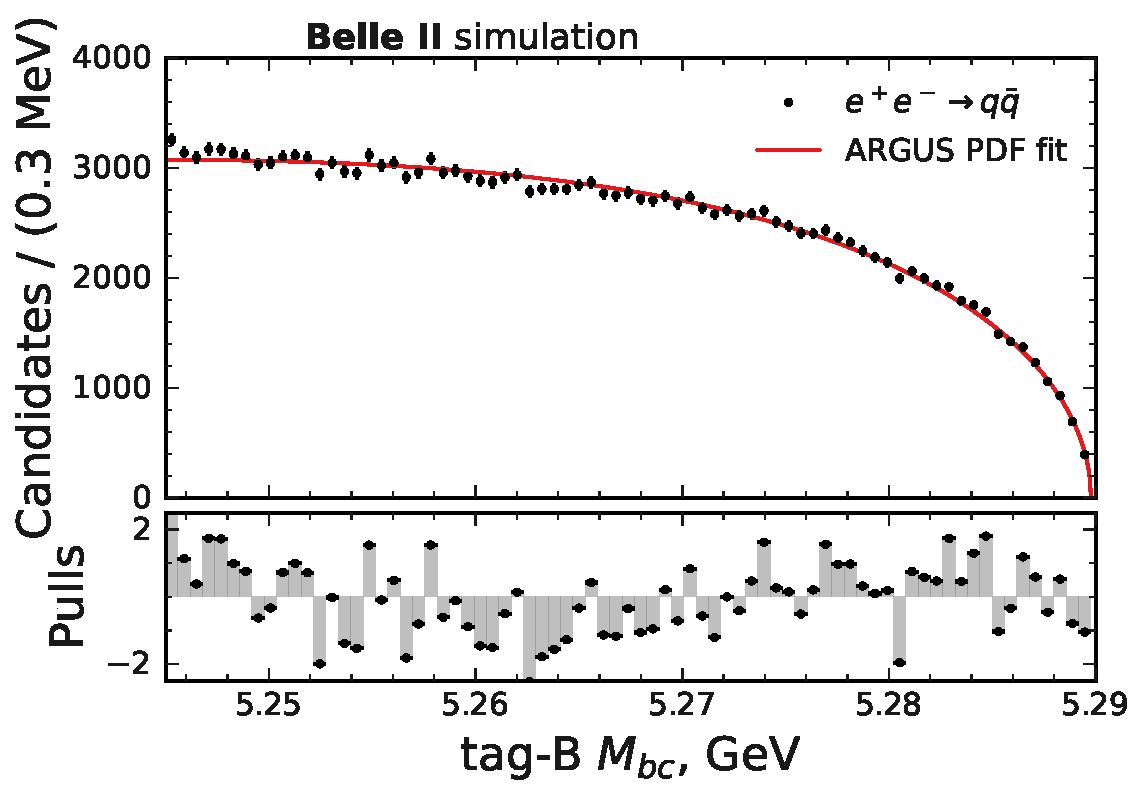
\includegraphics[width=0.3\textwidth]{figures/fitting/mbc_continuum_tags_fit.pdf}
    }
    \caption{\label{fig:tag_component_fits} Separate components that are present in generic \MC after selections that suppress background (\Cref{tab:cutflow}).
    The individual components are defined in \Cref{sec:fitting_components} text.
    Each distribution contains an unbinned illustrative fit to the data points, and the subpanels show the pull (XXXX) in each case.
    The fitting function for peaking tag \B mesons (\Cref{fig:good_tags_fit}) is chosen as the Crystal Ball function;
    for combinatorial tag \B mesons (\Cref{fig:combinatorial_tags_fit}) it is chosen as the 5th order Chebyshev;
    for continuum \epem\ra\qqbar events (\Cref{fig:argus_tags_fit}) it is chosen as the ARGUS function.
    }
\end{figure}
